%----------------------------------------------------------------------------
\chapter{Algoritmusok}
\label{sec:algoritmusok}
%----------------------------------------------------------------------------

%----------------------------------------------------------------------------
\section{Nemkorlátos optimalizáló algoritmusok}
%----------------------------------------------------------------------------

\subsection{Newton módszer}
A Newton módszer\footnote{Newton's method} alkalmas nemkorlátos differenciálható függvények gyökeinek a megtalálására. Ezt felhasználva, $f(x)=0$ helyett $g(x)=f'(x)=0$ egyenlet megoldásait keresve az $f$ függvény lokális szélsőértékeit találhatjuk me. Az iteráció egyes lépéseiben ehhez az alábbi képletet kell alkalmagznunk:
$$x_{n+1}=x_n-\gamma[Hf(x_n)]^{-1}\nabla f(x_n),$$ 
ahol $\gamma<1$ egy általunk megadható lépéshossz, $H$ a Hesse-mátrix, $\nabla f(x)$ pedig a gradiens.

A konvergálás várható ideje és iterációszáma nagyban függ attól, hogy az iteráció kezdőpontja mennyire esik közel a keresett gyökhöz. Jó esetben viszont nagyon gyorsan tud jó eredményt szolgáltatni.

Láthatjuk, hogy a mi esetünkben ez több kívánni valót is hagy maga után: szükséges hozzá a második derivált számítása minden iterációban, csak lokális szélsőérték keresést biztosít, és nincs lehetőségünk a korlátok kezelésére. Szerencsére azonban nem kell teljesen lemondanunk az algoritmusról, mivel több olyan megvalósítása is létezik, melyek lehetővé teszik olyan függvények optimalizálást, ahol a Hesse-mátrix nem áll rendelkezésünkre. Ezeket az algoritmusokat kvázi-Newton módszerekként emlegetjük.

\subsubsection{BFGS}
A feltalálóiról elnevezett Broyden-–Fletcher--Goldfarb--Shanno algoritmus egy a nagyon hatékony optimalizáló algoritmusok közül. A kvázi-Newton családba tartozó módszer a Hesse-mátrixot egy becsült mátrixszal közelíti, melyet minden iterációban a gradiens alapján frissít. Ezzel számítási költséget spórolhatunk. A módosított algoritmus a következő lépéseket hajtja végre, míg nem konvergálunk a megoldáshoz:
\begin{enumerate}
	\item $B_kp_k=-\nabla f(x_k)$ egyenlet megoldásával kiszámoljuk $p_k$ értékét, ahol $B_k$ mátrix a Hesse-mátrix közelítése, kezdeti értéke $B_0=I$ egységmátrix.
	\item Tetszőleges egydimenziós optimalizálással megkereshető az $f(x_k+\alpha p_k)$ függvény minimuma,
	\item amivel ezután $x_{k+1}=x_k+s_k$, ahol $s_k=\alpha _kp_k$.
	\item A becsült $B_k$ mátrixot a következő egyenlet alapján frissítjük, a gradienseket felhasználva:
	$$y_k=\nabla f(x_{k+1})-\nabla f(x_k), \quad B_{k+1}=B_k+\frac{y_ky_k^T}{y_k^Ts_k}-\frac{B_ks_ks_k^TB_k}{s_k^TB_ks_k}.$$
\end{enumerate}

Eggyel tovább fejlesztett verziója, a Limitált memóriájú BFGS (továbbiakban \mbox{L-BFGS}) pedig azt is biztosítja, hogy az iterációk során az átlagosnál jóval kevesebb memóriát használunk.

Az eredeti Newton módszernél megfelelőbb a mi céljainkra, mivel csak gradiens számítást igényel. A kezdőpont azonban itt is nagy hatással van az eredményre, és ebben az esetben sincsen biztosítva a globális optimalizálás.

\subsection{Gradiens módszer}

A gradiens módszer\footnote{Gradient descent} egy másik ismert megoldás az optimalizálásra. Arra a megfigyelésre alapul, hogy ha egy pontban a gradiens irányával ellentétes irányba megfelelően kis lépést teszünk, biztos, hogy a jelenlegi pontnál alacsonyabb helyre kerülünk. Megfelelően folytatva ezt a szekvenciát feltehetően egy lokális minimumba érkezünk. Az iterációs lépés tehát a következő:
\begin{equation}
	\label{eq:gd}
	x_{n+1}=x_n-\gamma _n\nabla f(x_n),\quad \textnormal{ahol}\quad \gamma _n=\frac{(x_n-x_{n-1})^T[\nabla f(x_n)-\nabla f(x_{n-1})]}{\|\nabla f(x_n)-\nabla f(x_{n-1})\|^2}.
\end{equation}
Tehát minden lépésben a lépés nagyságát is módosítjuk a gradiens és a mozgás függvényében. A lokális minimumba való konvergálás ilyen módon biztosítva van. 

Az általunk befolyásolható paraméter itt is a kezdőpont, máshonnan indítva az algoritmust más stacionárius pontot találhat meg.

\subsection{Részecske raj optimalizációk}

\begin{figure}
	\centering
	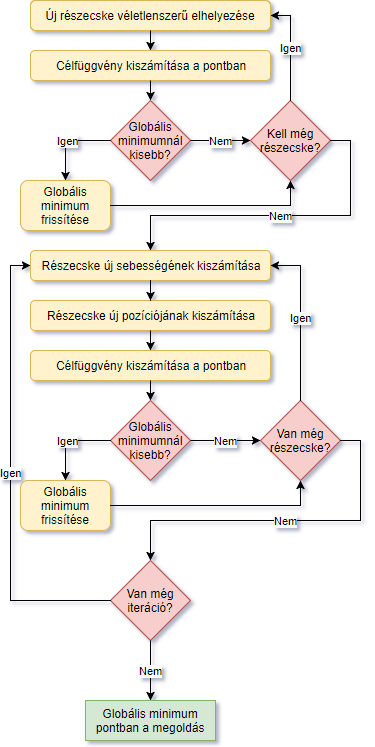
\includegraphics[height=200mm, keepaspectratio]{figures/pso.png}
	\caption{Részecske raj optimalizáció}
	\label{fig:pso}
\end{figure}
A részecske raj optimalizálás\footnote{Particle swarm optimization} során a keresési térben részecskéket veszünk fel. Ezek a részecskék egy egyszerű matematikai formula alapján járják be a teret, miközben a saját maguk és a globálisan ismert eddigi minimumhely ismeretében számolják ki minden iterációban, merre tegyék meg a következő lépést. A folyamatot \aref{fig:pso}. ábra szemlélteti. Az $i.$ részecske sebességének és pozíciójának kiszámításához használt képlet:
\begin{equation}
	\label{eq:pso}
	v_{i+1}=\omega v_{i}+\phi _pr_p(p_{i}-x_{i})+\phi_gr_g(g-x_{i}), \quad\textnormal{majd ezzel}\quad x_{i+1}=x_i+v_{i+1},
\end{equation}
ahol $r_p, r_g \sim U(0,1)$ véletlen számok, $\omega, \phi_p$ és $\phi_g$ pedig általunk választott hiperparaméterek. Ezeknek a megválasztása nagy körültekintést igényel, hisz jelentősen befolyásolják az algoritmus eredményességét.

Minden új pozíció kiszámításakor a részecske ellenőrzi, kisebb függvényértékű helyre érkezett-e, mint a lokálisan vagy globálisan ismert minimum, és ha igen, frissíti a megfelelő értékeket.

Az algoritmus futása során lényegében úgy mozognak a részecskék, hogy adott mértékben az ismert legalacsonyabb hely felé, adott mértékben pedig az általuk ismert legjobb hely felé próbálnak tartani, mindkét tényezőt egy véletlen számmal súlyozva. Sejthető, hogy ezzel semmilyen biztosítékot nem garantálhatunk a végeredményt illetően. Bár a gradiens számítását itt megspóroljuk, a sok részecskéhez tartozó függvényszámítások olyan nagyobb költséget okozhatnak, mint egy gradienst is használó, de kevesebb iteráció alatt konvergáló algoritmus. Kellő számú részecskével, kellő számú iteráció alatt viszont jó eredmény érhető el.

A tervező döntése a sebességek kiszámításában szereplő hiperparaméterek értéke, a részecskék és iterációk száma, illetve a tér azon részének a kiválasztása is, melyen a részecskéket elhelyezi. Ebből a térből a részecskék ki tudnak lépni, így a korlátok kezeléséhez plusz logika beépítése szükséges az algoritmusba.

\subsubsection{Méh algoritmus}
\begin{figure}
	\centering
	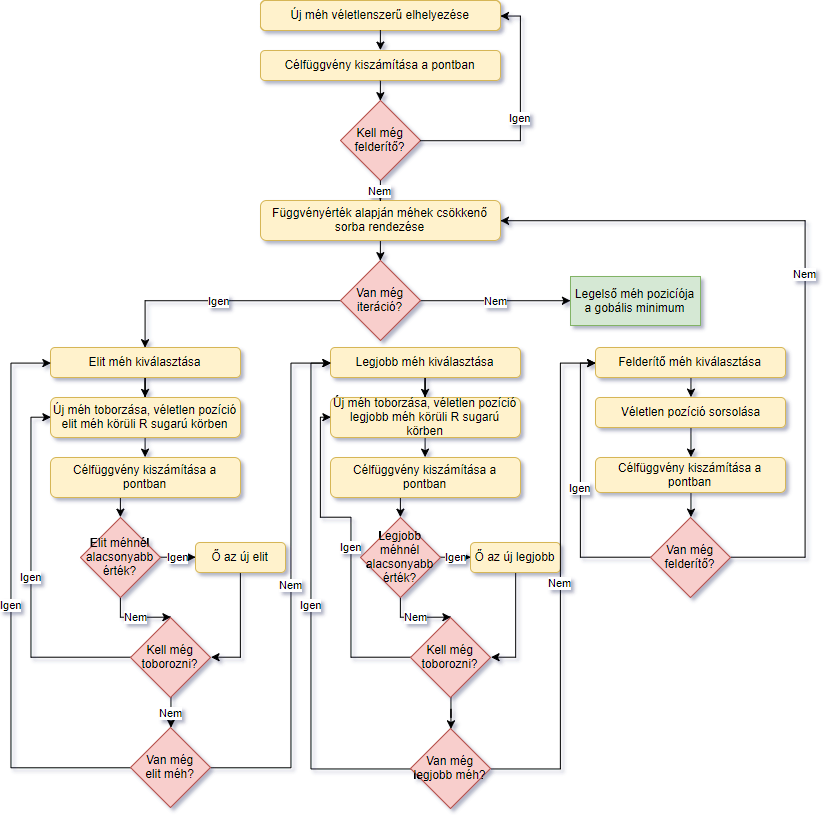
\includegraphics[width=150mm, keepaspectratio]{figures/bees.png}
	\caption{Méh algoritmus}
	\label{fig:bees}
\end{figure}

A természetben számtalan helyen visszaköszönnek a matematika szépségei. Rengeteg algoritmus mintázható az élőlények viselkedéséről vagy a természeti jelenségekről. Ezt teszi a méh algoritmus is. A részecske raj optimalizációk családjába tartozó módszer szintén nem használ deriváltszámítást, viszont a részecskék mozgása hierarchikusabb az alap algoritmus véletlenszerű mozgásánál. 

A méhek úgy keresik meg a lehető legtöbb virágot tartalmazó területeket, hogy először \textbf{felderítők}et küldenek véletlenszerű helyekre, majd visszaérkezésük után azok a méhek \textbf{toborozzák} magukhoz a legtöbb \textbf{segítőt}, akik a legjobb helyeket találták. A folyamatot \aref{fig:bees}. ábra szemlélteti.
Az első $b$ db, legjobb területet találó méhek a \textbf{lebjobb méhek}, azon belül az első $e$ db legjobbak az \textbf{elit méhek}. Értelem szerűen az elit méhek kapják a legtöbb segítőt maguk köré, a legjobbak, akik nem elitek, náluk kevesebbet. A többi toborzó marad véletlenszerű területek felderítőjének.

Minden iteráció során a segítő méhek egy $r$ sugarú körben véletlenszerűen helyezkednek el a toborzójuk által talált legjobb pont körül. Ezt a számot aztán iterációnként adott mértékben csökkenthetjük, így koncentrálva minél jobban az optimálisnak tűnő helyekre. Ha egy részecske az eddigi minimumnál jobb pontot talál, ő veszi át a toborzó szerepét, és az utána következő iterációban már hozzá viszonyítva helyezkednek el a többiek.

Így a biztatónak ígérkező területek jóval több részecske által kerülnek felderítésre, ezzel növelve a lehető legjobb terület megtalálásának valószínűségét. Azok a méhek, akik nem kerültek a legjobbak közé, folytatják véletlenszerű felderítésüket, ezzel biztosítva azt is, hogy van esélyünk az eddig esetleg elkerült globálisan optimális helyet is megtalálni.

Általunk megadandó hiperparaméterből van bőven:
\begin{itemize}
	\itemsep0em 
	\item felderítő méhek száma (toborzottakat nem beleszámítva) 
	\item legjobb méhek száma
	\item elit méhek száma
	\item legjobb méhek által toborzott méhek száma
	\item elit méhek által toborzott méhek száma
	\item iterációk száma
	\item a keresési terület határai
	\item a keresési kör sugara
	\item keresési kör csökkentésének mértéke
\end{itemize}

\subsubsection{Gradiens módszerrel ötvözve}

Sok esetben a célunk eléréséért nem egy, hanem egyszerre több algoritmus által nyújtotta lehetőségeket kell kihasználnunk. A részecske raj algoritmusok globális keresési tulajdonsága csábító, de hatékonysága csekély. Ellenben a gradiens módszer, bár biztosítja egy minimumhely megtalálását, ennek globális voltáról nincs információja.

Ideális megoldás lehet, ha a két ismert algoritmust ötvözzük. Ennek egy megvalósítása, ha minden iterációban a részecskék \aref({eq:pso}) képlet alapján kiszámolják az új pozíciójukat, majd az ezután ismert globális minimumhelyről indulva végzünk néhány lépést a gradiens módszerrel \aref({eq:gd}) képletek alapján. Ezáltal biztosíthatjuk a keresési tér bejárását globális optimum után kutatva, és az ígéretesnek tűnő pozíciókból nem kell a véletlenre bíznunk magunkat, hogy mennyire tudjuk megközelíteni a tényleges szélsőértéket, a gradiens használatával biztosra mehetünk. Arany középút, mely a költséges műveletet, a derivált számítást csak ott végzi el, ahol a legnagyobb a valószínűsége az optimális hely megtalálásának.

\subsection{Szimulált lehűtés}

Szintén egy természetből vett példát utánozó algoritmus a szimulált lehűtés\footnote{Simulated annealing}. Köztudott, hogy egy anyag részecskéi annál jobban mozognak, minél magasabb az anyag hőmérséklete. A hőmérséklet csökkenésével ez a mozgás lassul, míg végül ki nem alakul a szilárd anyagra jellemző szabályos kristályszerkezet.

Az optimalizáló algoritmusban a rendszerünket egy kezdeti hőmérsékletről indítjuk, és ezt minden iterációban meghatározott arányban csökkentjük. A jelenlegi pozíciónk körül egy $R$ sugarú körben kiválasztunk egy véletlenszerű pontot, majd eldöntjük, odaugrunk-e. Ez a döntés egy olyan valószínűséget adó egyenleten kell, hogy alapuljon, aminek az eredményéül magas hőmérséklet esetén nagy valószínűséggel a jelenleginél kedvezőtlenebb helyekre is átugrunk, a hőmérséklet csökkenésével azonban egyre kevésbé kockáztatunk. Ezzel csökkenthető annak az esélye, hogy egy lokális minimumba ragad a rendszer.
Valószínűséget adó egyenlet az én esetemben:
\begin{equation*}
f(x_{new},x_{old})=
\begin{cases}
	1 & x_{new}<x_{old}\\
	e^{\dfrac{x_{old}-x_{new}}{T}} & x_{new}\ge x_{old}
\end{cases},
\end{equation*}
ahol $T$ a rendszerünk jelenlegi hőmérséklete. Amennyiben a visszatérési érték nagyobb egy $r\sim U(0,1)$ eloszlású véletlen számnál, végrehajtjuk az ugrást. Ellenkező esetben nem változtatunk a pozíciónkon. Annak az érdekében, hogy több lehetőséget adjunk az ugrásra, beiktatható egy ciklus, hogy 2-3 alkalommal próbálkozzon a rendszer ugyanazon hőmérsékletén új pozícióba jutni.

Egyszerűsége miatt közkedvelt algoritmus, hiszen itt sincs szükség derivált számítására. Hasonlóan azonban az előzőekhez, a hiperparaméterek beállítása itt is nagy hatással lehet az eredményességre.

Általunk megadandó paraméter a kezdeti hőmérséklet, a hőmérséklet iterációnként való csökkentésének aránya, a keresés $R$ sugarának nagysága, és a csökkentésének az aránya.

%----------------------------------------------------------------------------
\section{Bayesi optimalizáció}
%----------------------------------------------------------------------------
A Bayesi optimalizáció módszere eltér az eddig megismert algoritmusokétól. Fix képletek helyett megpróbáljuk az iterációk során megtanulni a modellünk viselkedését, az eddigi kiértékelt pontok és a belőlük számított előzetes becslések alapján. Nagy számításigényű sztochasztikus rendszereink esetében ez egy ideális működés, mivel minimális kiértékelésre törekszünk azáltal, hogy a becslések alapján a legígéretesebbnek tűnő helyen számítjuk ki a függvényértéket.

\subsection{Gépi tanulás}

A gépi tanulás\footnote{Machine learning} a számítástudomány azon területe, mely képessé teszi a számítógépeket a tanulásra anélkül, hogy azt közvetlenül leprogramoznánk. Kapcsolódik a számítási statisztikákhoz, melyek célja előfeltételezések, jóslások számítása a rendszerhez, még a kiértékelése előtt. Többek között ezért a matematikai optimalizálásban is nagyon jó eszköznek bizonyult.

A kernel gépek a mintaelemzéses algoritmusok egy fajtája. Fő célja az adatok közötti kapcsolatok tulajdonságainak a vizsgálata és megismerése. Jellemzőjük, hogy tanulásuk során megjegyzik az összes eddigi bemenetüket és kimenetüket. Egy ismeretlen paraméterlekötés esetén annak kiértékelt értékét az ismert értékek és a kernel függvény segítségével becsülik meg.

\subsection{Gauss-folyamat}

A Gauss-folyamatok praktikus valószínűségi megközelítést nyújtanak a kernel gépekkel való tanuláshoz. Egy sztochasztikus folyamat valójában egy valószínűségi eloszlás -- mely leír egy véges dimenziójú véletlen valószínűségi változót -- általánosítása függvények egy lehetséges halmazaként. Azon folyamatokat, melyek esetében ez egy normális eloszlás, Gauss-folyamtoknak nevezzük.

Segítségükkel kétféle szempontból is vizsgálhatjuk a modelljeinket. A regresszió lehetővé teszi a célfüggvényünk alakjának modellezését, ami által minden iteráció során előfeltételezéssel élhetünk az ismeretlen helyek függvényértékeiről is, és ezt felhasználva irányíthatjuk az optimalizáló algoritmust. Egy ilyen predikciót szemléltet a \ref{fig:gp}. ábra, az eddig kiszámított pontok ismeretében a lehetséges illeszkedő függvények várható értékét véve. Ez a feltételezett modell minden újabb megismert ponttal módosul, precízebb és -- reményeink szerint -- valósághűbb lesz.

\begin{figure}[!ht]
	\centering
	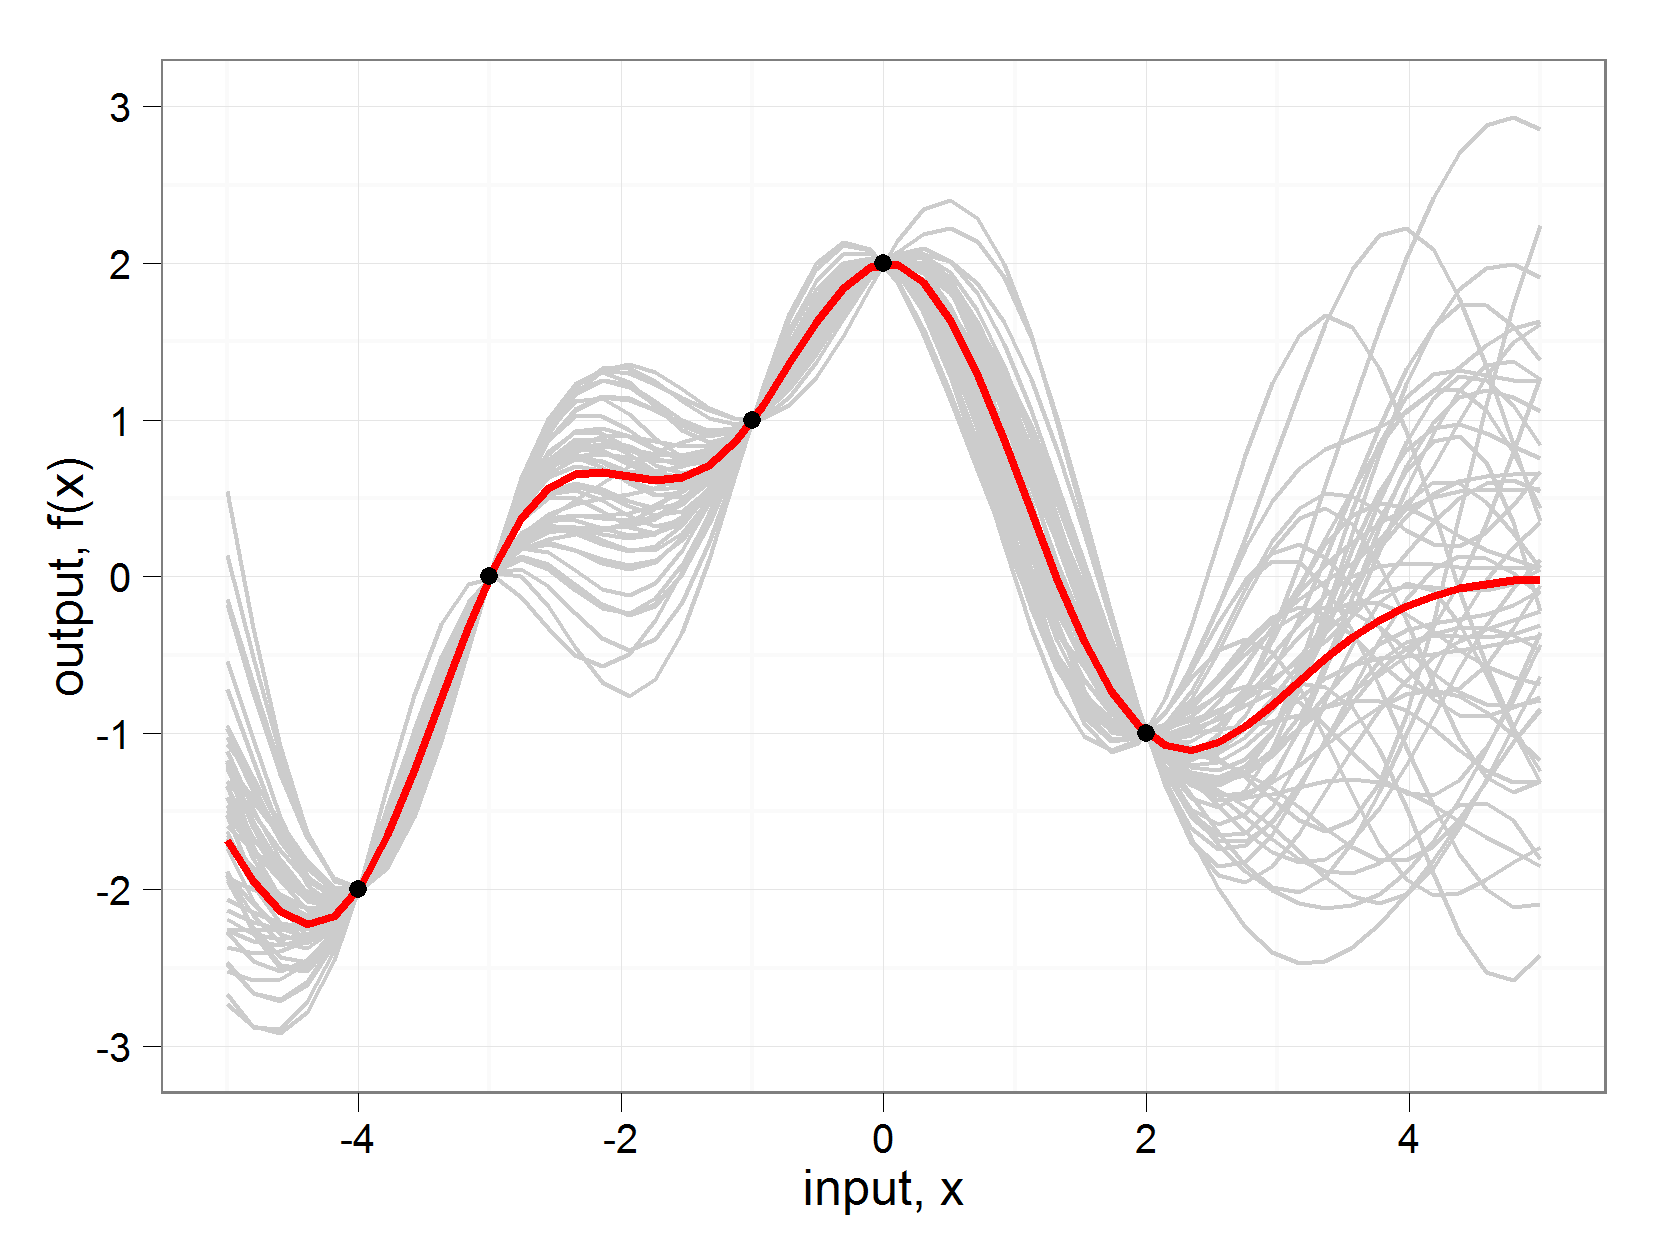
\includegraphics[width=140mm, keepaspectratio]{figures/gp.png}
	\caption{Gauss-folyamat regressziós becslése}
	\label{fig:gp}
\end{figure}

A klasszifikáció diszkrét osztályokba sorolja a tér pontjait. A mi esetünkben egy bináris osztályozásról beszélhetünk, azt tekintve, hogy az értelmezési tartomány adott pontján a megoldó keretrendszer által a modell kiértékelhető-e (1), vagy nem (-1). A regresszióhoz hasonlóan itt is minden iterációval frissítjük a becsült modellünket, melyet felhasználva következtetéseket vonhatunk le, a tér egyes területein valószínűleg értelmezhető-e a célfüggvényünk.\cite{GPKonyv}

\subsection{Bayesi optimalizáció}

\label{subsec:bayes}
A Bayesi optimalizáció egy olyan, függvények fölötti a posteriori\footnote{Tapasztalatból származó ismeret} eloszlással dolgozik, mely a legjobban leírja az optimalizálandó függvényt. Ahogy a megfigyelt értékek száma nő, a jósolt eloszlásunk úgy válik biztosabbá. Amint egyre nagyobb valószínűséggel tudjuk megállapítani, mely területek a legérdemesebbek az újabb iterációkra, és ezáltal a modell pontosabbá tételére, úgy válik az algoritmus egyre hatékonyabbá.

Az algoritmus működése egyszerű és nagyszerű, az alábbi lépéseket ismétli, míg nem teljesül a megállási feltétel. Ez általában a végzendő iterációk számára vonatkozik.
\begin{enumerate}
	\item Tesztpontokkal való kezdeti modell betanítása.
	\item Nyereség függvény\footnote{Acquisition function} maximumának megkeresése a modell alapján.
	\item Célfüggvény kiértékelése a talált helyen.
	\item Modell frissítése a kiértékelt ponttal.
\end{enumerate}

\subsubsection{Nyereség függvény}

A Gauss folyamat által felállított modell várhatóérték függvénye nem áll rendelkezésünkre zárt alakban, így nem tudunk róla semmilyen konkrét információt sem. A nyereség függvény használatával ezt a problémát át tudjuk hidalni az algoritmus futása során. 

A nyereség függvény az értelmezési tartomány pontjaihoz egy olyan értéket rendel, mely kifejezi, mennyire lenne hasznos az adott ismeretlen pontot kiértékelni a modell javítása érdekében, az ismert pontok értékeinek függvényében. Ennek a függvénynek a maximumát keressük, és itt fogjuk a következő kiértékelést elvégezni, az eredménnyel pedig a modellt frissíteni.

A tervező döntése a megfelelő nyereség függvény kiválasztása. Hasznos lehet többet is kipróbálni, esetleg ötvözni őket, hisz érthető módon ez is befolyásolhatja az algoritmus hatékonyságát.\\[3mm]
\textbf{Leggyakoribb nyereség függvények\cite{AcqFgvCikk}:}
\paragraph[Javulás valószínűsége]{Javulás valószínűsége\footnote{Probability of improvement}}
\begin{equation}
	\label{eq:POI}
	f_{PI}(x;\left\lbrace x_n,y_n\right\rbrace ,\theta)=\Phi(\gamma(x)), \qquad \gamma(x)=\frac{f(x_{best})-\mu(x;\left\lbrace x_n,y_n\right\rbrace ,\theta))}{\sigma(x; \left\lbrace x_n,y_n\right\rbrace ,\theta)},
\end{equation}
ahol $\left\lbrace x_n,y_n\right\rbrace$  kifejezés jelenti az eddig ismert pontokban a függvényértékeket, $\theta$ egy hiperparaméter mely a modellhez igazítandó, $\Phi$ a standard normális eloszlás függvénye, a  $\mu$ az aktuális modell váratóérték függvénye, $\sigma$ pedig a modell szórásfüggvénye.
\paragraph[Javulás várható értéke]{Javulás várható értéke\footnote{Expected improvement}}
\begin{equation}
	\label{eq:EI}
	f_{EI}(x;\left\lbrace x_n,y_n\right\rbrace ,\theta)=\sigma(x;\left\lbrace x_n,y_n\right\rbrace ,\theta)(\gamma(x)\Phi(\gamma(x))+\phi(\gamma(x)),
\end{equation}
ahol $\phi$ a standard normális eloszlás sűrűségfüggvénye (eloszlásfüggvény integrálja).
\paragraph[Alsó biztos határ]{Alsó biztos határ\footnote{Lower confidence bound}}
\begin{equation}
	\label{eq:LCB}
	f_{LCB}(x;\left\lbrace x_n,y_n\right\rbrace ,\theta)=\mu(x;\left\lbrace x_n,y_n\right\rbrace ,\theta)-\kappa \sigma(x;\left\lbrace x_n,y_n\right\rbrace ,\theta),
\end{equation}
ahol $\kappa$ hiperparaméter hivatott kifejezni a kizsákmányolás és felderítés módszere közötti egyensúlyozás mértékét, amiről bővebben a következő alfejezetben olvashatunk.

Ezek az ismert függvények esetében már a maximum megtalálása jóval egyszerűbb, mint az ismeretlen célfüggvényünk esetében. Egy alkalmas optimalizáló algoritmus -- akár a fentebb említettek közül -- jóval kisebb költséggel oldja meg, mint az eredeti problémát. Ebben rejlik tehát a Bayesi optimalizáció titka.

\subsubsection{Kizsákmányolás vagy felderítés}
A kizsákmányolás\footnote{exploitation} vagy felderítés\footnote{exploration} dilemmája ismert számos tudományterületen. Az optimalizálás során ugyanúgy hasznos az új tudás szerzése ismeretlen függvényterületekről, ahogy szükségünk lenne a már ismert tudás pontosságának, hatékonyságának növelésére is. Az algoritmus futása során nagy kérdés, mikor éri meg jobban egy olyan területről választani kiértékelendő pontot, ahonnan még nincsenek információink, és mikor válik nagyobb hasznunkra az eddig ismert, ígéretesnek tűnő területek precízebb feltérképezése, a globális minimum megközelítése érdekében.

Ez a döntés szerencsére a javulás valószínűsége (\ref{eq:POI}) és várható értéke (\ref{eq:EI}) nyereség függvényekben implicit kódolva van. Az alsó biztos határ (\ref{eq:LCB}) esetében azonban nekünk kell a $\kappa$ változóval döntést hozni a megfelelő arányról.

\subsubsection{Kernel függvény}
A kernel, vagy más néven kovariancia függvények szintén nagyban kihatnak a Bayesi optimalizáció eredményére. Mint fentebb említettem, a Gauss folyamat a priori eloszlások összessége függvények felett.
Egy 0 várható értékű modell esetén a kernel függvény teljes mértékben leírja a Gauss folyamat viselkedését.
Általános esetben azonban a folyamat a priorjainak simaságát, periodikusságát, izotrópiáját és állandóságát adja meg.

Sztochasztikus rendszereknél gyakran használt kernel függvények:
\begin{itemize}
	\item Exponenciális/Laplace: $exp(-\alpha\|x-y\|), \quad \alpha>0$.
	\item Négyzetes exponenciális: $exp(-\alpha\|x-y\|^2), \quad \alpha>0$.
	\item Gamma exponenciális: $exp(-\alpha\|x-y\|^\gamma), \quad \alpha>0, 0<\gamma\le1$.
	\item Matérn 1/2: $\sigma^2exp\left( -\frac{\|x-y\|}{\rho}\right)$. 
	\item Matérn 3/2: $\sigma^2\left( 1+\frac{\sqrt{3}d}{\rho}\right) exp\left(\frac{\sqrt{3}\|x-y\|}{\rho}\right)$.
	\item Matérn 5/2: $\sigma^2\left( 1+\frac{\sqrt{5}\|x-y\|}{\rho}\frac{5\|x-y\|^2}{3\rho^2}\right) exp\left(\frac{\sqrt{5}\|x-y\|}{\rho}\right)$.
\end{itemize}
A képletekben $\alpha$ az euklideszi távolság skálázó paramétere, $\gamma$ a gamma eloszlás alakját meghatározó paraméter, $\rho$ a kovariancia nemnegatív hiperparamétere.\\

Összességében láthatjuk, hogy a Bayesi optimalizáció törekszik a minimális számítási költségre, és számos ponton ad lehetőséget a tervezőnek a testre szabásra. Gradiens számítást sem igényel (habár léteznek már azzal kibővített megoldások a hatékonyság növelése érdekében). 
A korlátok algoritmusba kódolására is van lehetőség, amit a későbbiekben látni fogunk. 
A legnagyobb biztató jel azonban a klasszifikáció nyújtotta lehetőség a függvénytér azon területeinek a megbecsülésére, ahol a függvényérték a megoldó keretrendszer által kiszámítható.

